\documentclass[conference]{IEEEtran}
\IEEEoverridecommandlockouts
% The preceding line is only needed to identify funding in the first footnote. If that is unneeded, please comment it out.
\usepackage{cite}
\usepackage{amsmath,amssymb,amsfonts}
\usepackage{algorithmic}
\usepackage{graphicx}
\usepackage{textcomp}
\usepackage{xcolor}
\def\BibTeX{{\rm B\kern-.05em{\sc i\kern-.025em b}\kern-.08em
    T\kern-.1667em\lower.7ex\hbox{E}\kern-.125emX}}
\PassOptionsToPackage{hyphens}{url}\usepackage{hyperref}
\begin{document}

\title{Artificial Intelligence for Defence \\in an EQF6 Training and Education Program,\\ from the Design to the Execution
\thanks{This study was partly funded by the EU project ASSETs+ Project (Alliance for Strategic Skills addressing Emerging Technologies in Defence) EAC/A03/2018 - Erasmus+ programme, Sector Skills Alliances, Lot 3: Sector Skills Alliance for implementing a new strategic approach (Blueprint) to sectoral cooperation on skills G.A. NUMBER: 612678-EPP-1-2019-1-IT-EPPKA2-SSA-B.}
}

\author{\IEEEauthorblockN{E. Grivel}
\IEEEauthorblockA{
\textit{Bordeaux INP}\\
\textit{ENSEIRB-MATMECA}, Talence, France \\
eric.grivel@bordeaux-inp.fr}
\and
\IEEEauthorblockN{B. Pesquet}
\IEEEauthorblockA{
\textit{Bordeaux INP}\\
\textit{ENSC}, Talence, France \\
baptiste.pesquet@ensc.fr}\\
\IEEEauthorblockN{A. Zemmari}
\IEEEauthorblockA{
\textit{Univ. Bordeaux}\\
Talence, France \\
zemmari@u-bordeaux.fr}
\and
\IEEEauthorblockN{T.-B. Airimitoaie}
\IEEEauthorblockA{
\textit{Univ. Bordeaux}\\
Talence, France\\
tudor-bogdan.airimitoaie@ims-bordeaux.fr}
}

\maketitle
\begin{abstract}
In this paper, we present the main steps of the methodology we followed to design and prototype a module dedicated to artificial intelligence (AI) for Defence for students at the level 6 in the European Qualifications Framework (EQF). Based on a top-down approach for the design taking into account the market needs, this module is based on seasonal schools, project-based learning and invited speakers coming from the local ecosystem sharing their experiences with AI. This combination aims at attracting students to engineering in the field of Defence. Finally, it should be noted that a part of this module can be done in a hybrid way. \end{abstract}

\begin{IEEEkeywords}
Artificial intelligence, Defence, seasonal schools, invited speakers, project based learning.
\end{IEEEkeywords}

\section{Introduction}
Nowadays, Artificial Intelligence (AI) is everywhere in our everyday life. Its rise in healthcare is often motivated by the willing to accelerate diagnostics. In the field of entertainment and e-commerce, it has a strong impact since many suggestions are made in terms of films and series the users would like to watch or items well-suited to each customer. Many artworks can be created through the use of AI. In banking and finance, it can be used to detect fraudulent activity. AI is more and more useful for  automatic language processing including
syntactic analysis and machine translation. In some domains like Defence, AI is also of real interest and a key tool for different purposes: pattern detection and recognition, decision-making support, etc.

\noindent In 2018,  the European Defence skills partnership (EDSP) was launched and the members highlighted deficiencies of skills in emerging technologies such as AI.

\noindent Started in 2020, the ASSETS+ project, which stands for "Alliance for Strategic Skills addressing Emerging Technologies in Defence"  is an ERASMUS+ European project\footnote{More particularly, the type of project is an Erasmus+ Sector Skills Alliance for implementing a new strategic approach (Blueprint) to sectoral cooperation on skills.} the purpose of which is to build a sustainable human resources supply chain for the European Defence industry, in order to boost innovation by both attracting highly-skilled young workers and upskilling its employees.  The consortium brings together seven companies from the Defence industry, nine higher education institutes (HEI), four vocational educational and training (VET) providers, sectoral organizations and research centres, from eight countries (Denmark, France, Germany, Italy, Poland, Portugal, Spain and Sweden). See for more details: https://assets-plus.eu/.

\noindent The goals of the project are numerous. Among them:
\begin{itemize}
    \item Identifying the outdated, established, mature and emerging trends in technologies, based on a data driven approach using 500.000 documents from databases like scopus, C4ISRNET and the national initiative for cybersecurity education (NICE).
    \item Deducing the skills that are currently required in many fields such as robotics, autonomous systems, AI, cybersecurity, and C4ISTAR (standing for command and control, computer, communication, intelligence, surveillance, target acquisition and recognition).
    \item Defining the market needs and the corresponding job profiles.
    \item Designing and prototyping new education and training programs for Defence at three different levels from EQF4/5 to EQF 7\footnote{In the European Qualifications Framework (EQF), there are 8 levels, all defined by a set of descriptors indicating the learning outcomes relevant to qualifications at that level in any qualifications system. See https://europa.eu/europass/en/description-eight-eqf-levels.} for upskilling or reskilling students and workers. The mid-term goal is to attract highly-skilled students in the domain, train the future Defence sector workers and upskill the employees already working in the field.  To this end, a common methodology has to be followed to get an easy qualification in terms of European credit transfer and accumulation system (ECTS) credits, EQF level and European Skills/Competences, Qualifications and Occupations (ESCO) taxonomy. See Figure 1.
    \item Developing a European Defence qualification system covering pedagogical and technical aspects while complying with education requirements and industrial needs.
\end{itemize}

\noindent It should be noted that ASSETs+ is a member of the pact for skills, which is a shared engagement model for skills development in Europe. Through the pact for skills, the European Commission (EC) is bringing together companies, workers, national, regional and local authorities, social partners, cross-industry and sectoral organizations, education and training providers, chambers of commerce and employment services in order to create a culture of lifelong learning at work. The reader may refer to \text{https://ec.europa.eu} for more information.

\noindent In this paper, we present one of the modules that have been designed, prototyped and executed for EQF-6 students. It deals with AI for Defence and combines different types of pedagogical activities: seasonal schools with invited speakers coming from the local eco-system and project-based learning.\\

\noindent The remainder of this paper is organized as follows. In section II, the design methodology that we used is described. In section III, details about the module are given. Finally, in section IV, a feedback and testimonies are provided.
\begin{figure}[htb]
    \centering
    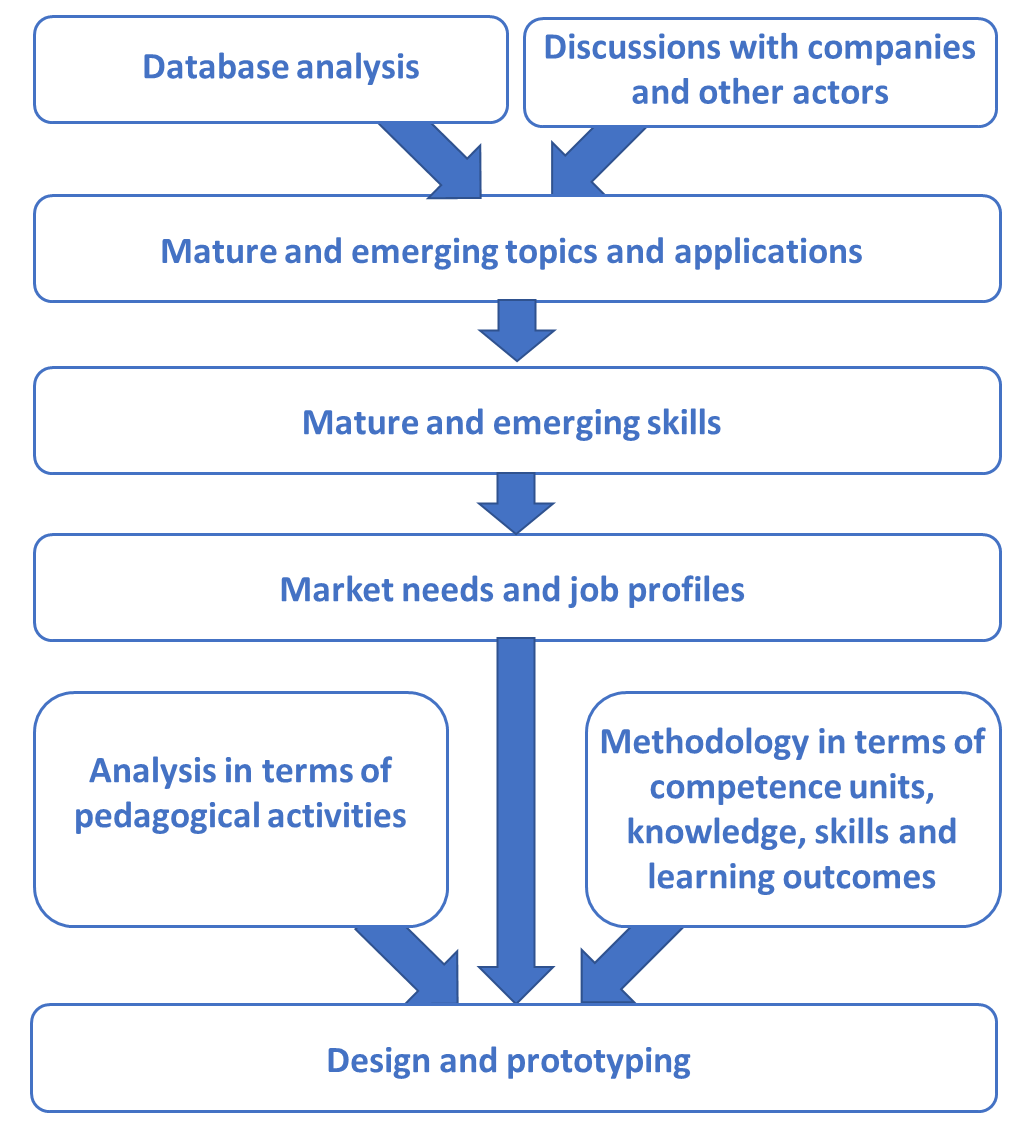
\includegraphics[width=\columnwidth]{timeflow_assetseqf6.png}
    \caption{Timeline of the design and prototyping of the EQF training and education program}
\end{figure}
%\subsection{Some concerns about the pedagogical activities}
\section{Design methodology used for the module}
The first step of the methodology we followed was to make a list of the pedagogical approaches that could be well suited to develop Defence-related skills needed in Europe. To this end, some workshops were organized to present some pedagogical approaches already implemented or existing learning environments. Among them, pedagogical activities based on "cooperative learning", "team working" or "group working" are known to increase interaction among students, to increase productivity and to improve critical thinking, self-esteem and positive inter-personal relationships \cite{b00}. In addition, some teaching formats facilitating cooperation between university and companies such as camp events, hackathons, prizes and contests, challenge based learning (CBL) and project-based learning (PBL) tackling complex problems can be very useful and serve as catalysts for future innovation. The reader may refer to \cite{b000,b0bis,b0ter,boq} for instance. Moreover, open innovation labs can be areas where university and industry can collaborate on common issues for creating, elaborating and prototyping solutions.

\noindent We also took advantage of experiences shared by colleagues such as \cite{bimp} in order to optimize the learning of heterogeneous classrooms.

\noindent When starting the design, our motivations were numerous: taking into account the market needs, improving the synergies between academia and industry in the domain, designing pedagogical activities encouraging students to respect a work ethic, developing an entrepreneurial spirit, fostering creativity and innovation and encouraging intercultural awareness and individual responsibility. 
Indeed, our purpose was to develop a skill-based approach where the concepts of knowledge and competency are clearly distinguished. Thus, knowledge corresponds to the learning foundation while the competency is a set of general and specific knowledge, know-how, and life skills used to solve a problem. Students must hence be embedded in an environment in which they have to learn how to use and apply knowledge.

\noindent If lectures remain one of the pillars in training programs, other pedagogical activities must be added in order to introduce the context and to present the applications as well as the issues related to the Defence sector so that the students can have a more concrete vision of the topic.

\noindent To this end, seminars in which different actors of the domain coming from the industry or clusters was one of the suggestions we kept in mind. Moreover, project-based and problem-solving activities as well as seasonal schools were also considered as relevant pedagogical tools to be deployed.  
\subsection{Guidelines to be followed}
We followed a guideline to design the training program in compliance with EQF, the ECTS and ESCO taxonomies.

\noindent The approach we had was to design competence units (CUs), corresponding to a set of modules of qualifications, consisting of a coherent set of knowledge and skills. The latter are written in terms of learning outcomes which express what the students know, understand and are able to do at the end of a learning process. The way these learning outcomes are written must be in line with what is expected at the EQF level. In other words, it is written with specific descriptors defined in terms of knowledge, skills and autonomy-responsibility. Thus, for EQF 6 level, the students must demonstrate advanced knowledge of the field. This involves a critical understanding of the theories and the principles that have been presented. In addition, the students have to demonstrate their interest for innovation and their ability to solve complex problems. Finally, regarding responsibility and autonomy, the students are expected to manage complex technical or professional activities or projects, taking responsibility for decision-making in unpredictable work or study contexts. In addition, they should be able to take responsibility for managing professional development of individuals and groups. 
\subsection{Application of this methodology for a module dedicated to AI for Defence}
In terms of prerequisites, the students are assumed to have basics in mathematics and programming and are expected to speak and read English.

\noindent In terms of knowledge, the objective was to create a module giving students advanced knowledge and critical understanding of the theory, principles and applicability of: 
\begin{itemize}
    \item Machine Learning (ML) overview,
    \item Model training and evaluation, 
\item Core ML algorithms. 
\item 
ML issues and set of practices making it possible to deploy and maintain ML models in production reliably and efficiently (MLops).
\end{itemize}
In terms of skills, the trainees should be able to: 
\begin{itemize}
    \item Prepare datasets for training, \textit{i.e.} be able to gather, analyse and pre-process real-world data to train ML models upon. 
\item Build ML models on various data types, \textit{i.e.} be able to train models that will be able to infer useful results from training data. 
\item Use standard Python libraries for ML, \textit{i.e.} be able to know and efficiently use the essential tools of the Python ML landscape. 
\item Understand the benefits and limits of ML approaches, \textit{i.e.} be able to choose between a ML-based approach and a traditional rule-based one depending on the project context and objective. 
\item Apply ML wisely, in accordance with ethical rules, \textit{i.e.} be able to understand and take into account the potential social and societal impacts of AI. 
\end{itemize}
From a design point of view, this led to a module with 42 contact hours. It should be noted that the students are assumed to spend approximately the same amount of time on their own. This follows the standard recommendations. The total workload is 80 hours. As 1 ECTS credit usually corresponds to 25h of total workload, 3 ECTS credits can be delivered.

\noindent \textit{Remark:} It could be recommended to have other CUs in the whole training program: one dedicated to mathematics for data science dealing with introduction and review of probability and statistics, basics in information theory, review of linear algebra and optimization methods.  Another CU should be related to programming in which 
programming environments, algorithmic structures, data structures and object-oriented programming are addressed. The last one can be dedicated to signal processing for ML in which the students learn some concepts dealing with signal and image processing\footnote{When dealing with AI, the data that are used are often signals recorded by sensors and images collected by cameras. The user must be able to pre-process these data and choose the best way to represent them (in the time/frequency/time-frequency domain or by using a set of features for instance.}, Markov decision processes and signal and image processing for ML.

\noindent Let us now focus our attention on the module dedicated to ML which addresses different concepts related to ML, from a general introduction to its application in the Defence sector through state-of-the-art techniques and tools. As depicted in Figure 2, the module is composed of three seasonal schools lasting from 2 to 3 days. During them, invited speakers coming from the AI for Defence ecosystem put in perspective the topics at hand.
A project-based learning activity acts as a common thread for students to apply their new knowledge and skills. 
\begin{figure}[ht]
    \centering
    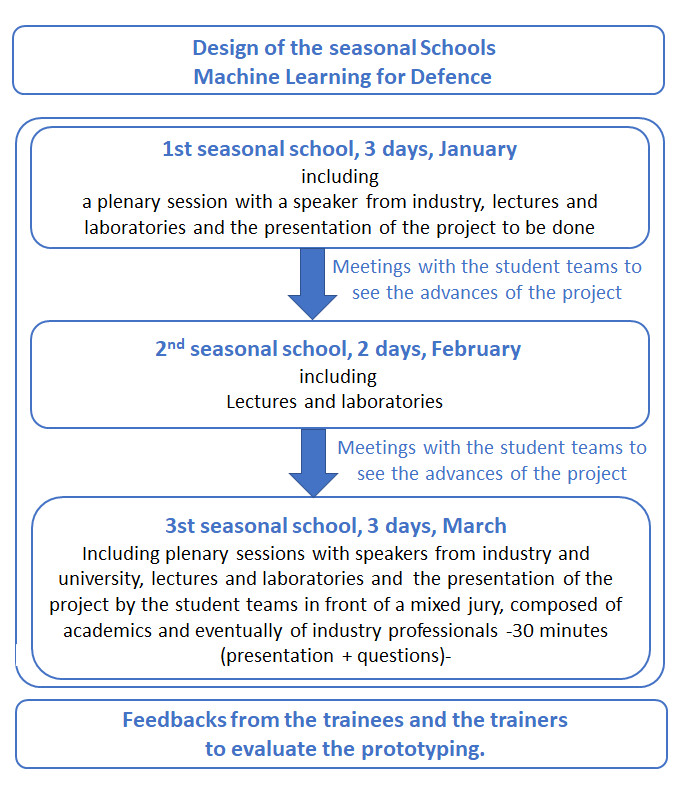
\includegraphics[width = \columnwidth]{assetsscpbl.png}
    \caption{Timeline of the seasonal schools}
\end{figure}
\section{From the design to the prototyping}
In this section, different aspects are presented when moving from the design phase to the prototyping phase.
\subsection{About invited speakers}
We found it interesting to ask different actors to speak of AI. Thus, engineers from companies such as Airbus and Thales located in the regions "Nouvelle Aquitaine" and "Occitanie" were invited to share some examples of applications of AI. Students are always very interested in having guest speakers from industry. They can project themselves on the uses and on the work that is done in a professional setting. Big companies are not the only ones to use AI. Therefore, a researcher from University of Bordeaux was also invited to give a talk about some complementary concepts of AI and its use. Note that SMEs could be also invited to share their own experience.
\subsection{About the project-based learning approach, from data to the oral defence}
One of the challenges we faced was to define the subject of the project that the students had to carry out. The first point was to choose a topic describing a situation that the students could easily understand or relate to their everyday life. "Realism" is a key point. The topic
had to be Defence-related and to have sufficient depth in order to offer room for various approaches and multiple solutions. Moreover, it had to push students to formulate different solutions and decide which one was the most suited.
Finally, when dealing with AI approaches, we are often led to process data. Our initial wish was to have data provided by companies in the Defence sector. However, within a company, this data may be of economic and/or strategic value. Its leakage and subsequent fraudulent use would be detrimental to them. Therefore, the provision of this sensitive set of data and their sharing with the students would have required numerous administrative procedures and were not without risk. The key points were to guarantee secure transfer and storage and then to ensure the `"proper" use of the data (no illegal copying, etc.) by the students. Of course, pre-processing data by removing sensitive information  could have been done by the industrial partners, but this would have taken a lot of time. We could also have asked the students to sign a document. Even if this can make students aware of good practices to adopt in terms of exchanging data with third parties, our wish was to facilitate the implementation of the project as much as possible. Consequently, the pedagogical team decided to define a project, avoiding the above problems by relying on a publicly available dataset.

\noindent Thus, the project of the seasonal schools focused on the detection of malware on mobile devices. The underlying idea was to embark students on a (cyber-) Defence-oriented task of intermediate difficulty. In order to apply the ML principles and use the tools discovered during the seasonal schools, the CCCS-CIC-AndMal-2020 dataset from \cite{b1,b2,b3} was used. It includes 200K benign and 200K malware samples totalling to 400K Android apps with 14 prominent malware categories and 191 eminent malware families. The goal of the project was to train models on this dataset so that they could classify never-seen-before mobile applications as either benign or harmful. Malware properties in the training set include both static features (app metadata, requested permissions, etc.) and dynamic features recorded by executing them in a sandboxed environment (memory usage, network access requests, system API calls, etc.). Malware status (benign or harmful) is also defined for each sample, making it possible to train models in a supervised fashion.

\noindent The three in-person seasonal schools were designed around this project (see the timeline in Figure 2 above):
\begin{itemize}
\item During the first one, the project and its goals were introduced to the students. They organised themselves as teams of two people and began toying around with the dataset. The malware identification objective being rather easy to understand, most questions were about the data: What is the business meaning of this particular feature? Which one is the target the model will have to predict? etc. By the end of the first school, all teams had (or at least, were expected to have) the required amount of knowledge, skills and understanding to start working on the project on their own.
\item The second seasonal school was associated to an intermediate milestone: being done with context understanding, objective definition, technical environment setup and dataset analysis, all mandatory steps to successfully train any ML model. During this seasonal school, student teams began the training step of the ML workflow.
\item The third seasonal school was used by teams to refine the training process, streamline their code and evaluate the performance of the models. During the last day, each team showcased its results and answered the questions of the jury members during a 20-minutes long oral defence. Juries included regular teachers already knowing the students. Other members could be invited in the future such as the members of the ASSETs+ consortium or local industrial partners.
\end{itemize}

\noindent The time interval between the seasonal schools varied from two to three weeks, during which personal work on the project was expected. A few days before the second and third schools, online meetings between student teams and a member of the pedagogical team took place. Their rationale was to assess results, answer questions and maintain the project rhythm between in-person sessions.

%\textcolor{green}{Baptiste, Tudor et Akka, merci de donner des éléments sur le projet : le titre et son objet ; comment les groupes se sont organisés en équipe ? quand le sujet a été donné ? comportement des élèves sur l'appropriation du sujet ? réunion intermédiaire entre équipe projet et enseignants ? organisation de la soutenance : durée, question, jury ?}

\subsection{Additional information}
We took into account the fact that when the students are comfortable with the instructor thanks to his/her warmth and empathy, the students are more willing to learn, participate and share in the learning environment \cite{b0}. 

\noindent The students had the freedom to choose their pair. This facilitated exchanges between them, even if they know each other for having been in class together. For this type of project, it seemed more relevant that the choice belong to them (motivation of each, involvement in the work, etc.).

\noindent At the end of the last seasonal school, a friendly moment was proposed during which the students could discuss with the organizing team around a coffee and small cakes.

\section{Feedback}
In this section, we share some feedback of students who participated in the seasonal schools.\\ \\
Kylian Deville, Student in the field of ISC - Complex systems Engineering:

\noindent \textit{“In my opinion, the seasonal schools are a good way to improve and reinforce the link between our studies and the professional world. Indeed, this prototype program allowed us to discover and learn new functionalities, and to acquire new knowledge concerning ML, which can be relevant for our future work.”}\\ \\
Hugo Zbinden, Student in the field AM2AS Automation and Mechatronics, Automotive, Aeronautics and Space:

\noindent \textit{“The fact that Machine Learning can be used almost anywhere is really great. I immediately tried to make a link between what we learned in class, and what we learned in the seasonal schools. The thing I liked the most personally during the seasonal schools was the plurality of aspects we worked on Machine Learning. It was not only programming but also data pre-processing, and even the ethical issues surrounding Machine Learning. We really learned to take a step back and critically look at our data, before trying to apply any Machine Learning algorithm on them.”}\\ \\
Daniel Camacho, Student in the field of AM2AS - Automation and Mechatronics, Automotive, Aeronautics and Space:

\noindent \textit{“Besides the content of the classes that we took, I think that one of the features that made the seasonal Schools so interesting, was its condensed format. Having classes three days in a row per month and being followed up by the trainers is just a very innovative way to learn several subjects in so little time. However, the thing that I have appreciated the most were the lectures with professionals in the field. Having the opportunity to exchange with people that are working on the subjects that we learned in class is just an excellent way to put in context the knowledge that you are receiving.”}

 \section{Conclusions and perspectives}
The module that has been designed and experimented with students at University of Bordeaux deals with artificial intelligence for Defence. Composed of seasonal schools lasting two to three days, it also includes a project. This pedagogical activity is also characterized by invited speakers working in the field of AI. We noticed that this combination was a real incentive to raise the attention of the students to the topic but also to the field of Defence.

%\section*{References}

\begin{thebibliography}{00}
\bibitem{b00}
L.~B.~Nilson, "Teaching at its best: A research-based resource for college instructors" 3rd edition, San Francisco, CA: Jossey-Bass, 2010.
\bibitem{b000} K.~Kohn Rådberg, U.~Lundqvist, J.~Malmqvist and O.~Hagvall
Svensson, "From CDIO to challenge-based learning experiences – expanding student
learning as well as societal impact? (2020), European Journal of Engineering Education, Vol. 45, n°1, pp. 22-37, 2020. DOI:
10.1080/03043797.2018.1441265
\bibitem{b0bis} Isabelle Liotarda and Valérie Revest, "Contests as innovation policy instruments: Lessons from the US federal
agencies' experience", Technological Forecasting and Social Change, Vol. 127, pp. 57-69, 2018.
\bibitem{b0ter} J.-R. Falleri, E. Grivel and L. Réveillere, "What can industrial partnerships bring to small-group projects to teach signal and image processing?" Eurasip conference EUSIPCO,  pp.~1786-1790, Aug 2015, DOI : 10.1109/EUSIPCO.2015.7362691.
\bibitem{boq} M.~Hernandez-de-Menendez, A.~Vallejo Guevara, J.~C. Tudon Martinez, D.~Hernandez Alcantara and R.~Morales‑Menendez, "Active learning in engineering education. A review of fundamentals,
best practices and experiences", International Journal on Interactive Design and Manufacturing (IJIDeM),  Vol. 13, pp. 909–922, 2019, https://doi.org/10.1007/s12008-019-00557-8
\bibitem{bimp} R. Kanth Aluvalu, V. Kulkarni and M. Asif, "Handling Classrooms with Students having Heterogeneous Learning Abilities", Journal of Engineering Education Transformations,
Vol. 31 , Oct. 2017, ISSN 2349-2473, eISSN 2394-1707
\bibitem{b1} A.~Rahali, A.~H.~Lashkari, G.~Kaur, L.~Taheri, F.~Gagnon, and F.~Massicotte, "DIDroid: Android Malware Classification and Characterization Using Deep Image Learning", 10th International Conference on Communication and Network Security (ICCNS2020), pp.~70–82, Tokyo, Japan, November 2020.
\bibitem{b2} D.~S. Keyes, B.~Li, G.~Kaur, A.~H. Lashkari, F.~Gagnon and F.~Massicotte, "EntropLyzer: Android Malware Classification and Characterization Using Entropy Analysis of Dynamic Characteristics", Reconciling Data Analytics, Automation, Privacy, and Security: A Big Data Challenge (RDAAPS), IEEE, Canada, ON, McMaster University, 2021.
\bibitem{b3} CCCS-CIC-AndMal-2020 dataset,\\ \url{https://www.unb.ca/cic/datasets/andmal2020.html}
\bibitem{b0} J.~Cornelius-White, "Learner-Centered Teacher-Student Relationships Are Effective: A Meta-Analysis",
 Review of Educational Research Vol. 77, n°1, pp.~113-143, March 2007, DOI:10.3102/003465430298563.
\end{thebibliography}

\end{document}
